%%%%%%%%%%%%%%%%%%%%%%%%%%%%%%%%%%%%%%%%%
% Short Sectioned Assignment
% LaTeX Template
% Version 1.0 (5/5/12)
%
% This template has been downloaded from:
% http://www.LaTeXTemplates.com
%
% Original author:
% Frits Wenneker (http://www.howtotex.com)
%
% License:
% CC BY-NC-SA 3.0 (http://creativecommons.org/licenses/by-nc-sa/3.0/)
%
%%%%%%%%%%%%%%%%%%%%%%%%%%%%%%%%%%%%%%%%%

%----------------------------------------------------------------------------------------
%	PACKAGES AND OTHER DOCUMENT CONFIGURATIONS
%----------------------------------------------------------------------------------------

\documentclass[paper=a4, fontsize=11pt]{scrartcl} % A4 paper and 11pt font size

\usepackage[T1]{fontenc} % Use 8-bit encoding that has 256 glyphs
\usepackage{fourier} % Use the Adobe Utopia font for the document - comment this line to return to the LaTeX default
\usepackage[spanish]{babel} % English language/hyphenation
\selectlanguage{spanish}
\usepackage[utf8]{inputenc}
\usepackage{amsmath,amsfonts,amsthm} % Math packages
\usepackage{graphicx}

\usepackage{sectsty} % Allows customizing section commands
\allsectionsfont{\centering \normalfont\scshape} % Make all sections centered, the default font and small caps

\usepackage{fancyhdr} % Custom headers and footers
\pagestyle{fancyplain} % Makes all pages in the document conform to the custom headers and footers
\date{}
\fancyhead{} % No page header - if you want one, create it in the same way as the footers below
\fancyfoot[L]{} % Empty left footer
\fancyfoot[C]{} % Empty center footer
\fancyfoot[R]{\thepage} % Page numbering for right footer
\renewcommand{\headrulewidth}{0pt} % Remove header underlines
\renewcommand{\footrulewidth}{0pt} % Remove footer underlines
\setlength{\headheight}{5.6pt} % Customize the height of the header

\numberwithin{equation}{section} % Number equations within sections (i.e. 1.1, 1.2, 2.1, 2.2 instead of 1, 2, 3, 4)
\numberwithin{figure}{section} % Number figures within sections (i.e. 1.1, 1.2, 2.1, 2.2 instead of 1, 2, 3, 4)
\numberwithin{table}{section} % Number tables within sections (i.e. 1.1, 1.2, 2.1, 2.2 instead of 1, 2, 3, 4)

\setlength\parindent{0pt} % Removes all indentation from paragraphs - comment this line for an assignment with lots of text

%----------------------------------------------------------------------------------------
%	TITLE SECTION
%----------------------------------------------------------------------------------------

\newcommand{\horrule}[1]{\rule{\linewidth}{#1}} % Create horizontal rule command with 1 argument of height

\title{	
\normalfont \normalsize 
\textsc{UNIVERSIDAD DE CANTABRIA, DEPARTAMENTO DE FÍSICA MODERNA} \\ [20pt] % Your university, school and/or department name(s)
\horrule{0.5pt} \\[0.4cm] % Thin top horizontal rule
\huge Física de Partículas Elementales (G71) \\ % The assignment title
\normalsize 4 Curso - Grado de Física (29 de Enero de 2019)
\horrule{2pt} \\[0.5cm] % Thick bottom horizontal rule
}

\begin{document}

\maketitle % Print the title

\vspace{-2.5cm}

%----------------------------------------------------------------------------------------
%	PROBLEM 1
%----------------------------------------------------------------------------------------
\textbf{Cuestión 1.} En Teorías de Gran Unificación (en inglés GUT) el protón no es estable y decae de la forma: $p^{+}\rightarrow\pi^{0} + e^{+}$. Asumiendo que la masa del positrón puede despreciarse
en comparación con las masas del protón y el pion ($m_{e^{+}}=0$), calcula la expresión para el momento del pion en el sistema de reposo del protón. \textbf{(1 Punto)}. Un electrón con una energía de 20 MeV colisiona con un
positrón en reposo dando lugar a dos fotones: $e^{-} + e^{+}\rightarrow\gamma + \gamma$. Si uno de los fotones es detectado formando un ángulo de 45 grados con la dirección inicial del electrón, ¿cuáles son las energías de los fotones 1 y 2 respectivamente?.
Considera una masa del electrón $m_{e^{-}} = 0.5 MeV$. \textbf{(1 Punto)}.
\\
\\
%----------------------------------------------------------------------------------------
%	PROBLEM 2
%----------------------------------------------------------------------------------------
\textbf{Cuestión 2.} Considera los operadores de proyección $P_{R} = \frac{(1+\gamma^5)}{2}$ y $P_{L} = \frac{(1-\gamma^5)}{2}$. Explica qué papel juegan en la descripción de la fuerza débil y cómo se relacionan con la quiralidad y la helicidad. \textbf{(0.5 Puntos)}. Demuestra que
$P_{L}\gamma^{\mu} = \gamma^{\mu}P_{R}$ y $P_{R}\gamma^{\mu} = \gamma^{\mu}P_{L}$. \textbf{(0.5 Puntos)}. Demuestra que si llamamos $\Psi_L = P_L\Psi$ y $\Psi_R = P_R\Psi$ entonces los adjuntos de $\Psi_L$ y de $\Psi_R$ cumplen
$\overline{\Psi_L} = \overline{\Psi}P_R$ y $\overline{\Psi_R} = \overline{\Psi}P_L$. \textbf{(0.5 Puntos)}. Demuestra también que $\overline{\Psi_L}\gamma^{\mu}\Phi_L = \overline{\Psi}\gamma^{\mu}P_L\Phi$. \textbf{(0.5 Puntos)}. 
%----------------------------------------------------------------------------------------
\\
\\
%----------------------------------------------------------------------------------------
%       PROBLEM 3
%----------------------------------------------------------------------------------------
\textbf{Cuestión 3.} Considera el siguiente proceso de aniquilación $q^{-}q^{+}\rightarrow\mu^{-}\mu^{+}$. Dibuja los dos posibles diagramas de Feynmann de 2 vértices que describen este proceso. \textbf{(0.5 Puntos)}. Indica
la estructura que tendría el elemento de matriz asociado a cada uno de ellos, explicando las diferencias. \textbf{(0.5 Puntos)}. Si el experimento en el que se está estudiando este proceso tiene una energía centro de 
masas $\sqrt{s}=20 GeV$: ¿Cuál de los dos será dominante?. Razona tu respuesta. \textbf{(1 Punto)}.  
%----------------------------------------------------------------------------------------
\\
\\
%----------------------------------------------------------------------------------------
%       PROBLEM 4
%----------------------------------------------------------------------------------------
\textbf{Cuestión 4.} Define los siguientes conceptos: Tasa de desintegración, Elemento de Matriz $|T_{fi}|$, Elemento de Matriz $|M_{fi}|$, Sección eficaz y Sección eficaz diferencial. \textbf{(1.0 Puntos)}. Indica para cada una
de estas cantidades si se trata de una cantidad invariante bajo transformaciones de Lorenz o no. \textbf{(0.5 Puntos)}. La tasa de desintegración para el decaemiento de una partícula en otras dos $A\rightarrow B + C$, en
el sistema de reposo de la partícula A, viene dado por: $\Gamma = \frac{|\vec{p^{*}}|}{32\pi^2m_i^2} \int |M_{fi}|^2 d\Omega$. Explica a qué nos referimos con el momento $\vec{p^{*}}$, cuál sería su ecuación en términos de las masas de las partículas y cómo se relaciona con la expresión integral de la densidad de
estados. (\textbf{Nota:} No es preciso despejar el momento, basta con indicar la ecuación que cumple.)\textbf{(0.5 Puntos)}.
\\
\\
%----------------------------------------------------------------------------------------
%       PROBLEM 5
%----------------------------------------------------------------------------------------
\textbf{Cuestión 5.} Madame Wu diseñó un experimento en el que un núcleo de cobalto decae en un núcleo de níquel, un electrón y un antineutrino: $Co\rightarrow Ni + e^{-} + \bar{\nu_e}$ en presencia de un campo magnético. El diagrama \ref{dibujo}
muestra un esquema de este proceso para dos situaciones en las que el campo magnético está alineado (derecha) o antialineado (izquierda) con el eje Z. En ambos casos el spin del cobalto y del níquel se alinea siguiendo el campo magnético. Puesto que el níquel tiene 
una unidad menos de spin que el cobalto, el electrón y el anti-neutrino tendrán que compensar la pérdida de spin tal y como se indica en el diagrama. Asigna y calcula los espinores de Dirac autoestados de la helicidad \ref{espinores} a cada uno de los electrones y anti-neutrinos en el diagrama, en función del momento $p$ y las masas (asume $\phi=0$). \textbf{(0.5 Puntos)}. Asumiendo que la masa del neutrino es exactamente 0, uno de los diagramas tiene una probabilidad de ocurrir igual a 0. Indica cuál y explica por qué en relación al elemento de matriz asociado a la fuerza débil mediada por un bosón W. \textbf{(0.5 Puntos)}. Usando los espinores de Dirac y los operadores de proyección quiral demuestra lo mismo matemáticamente. \textbf{(1 Punto)}.  

\begin{figure}[!h]
\begin{center}
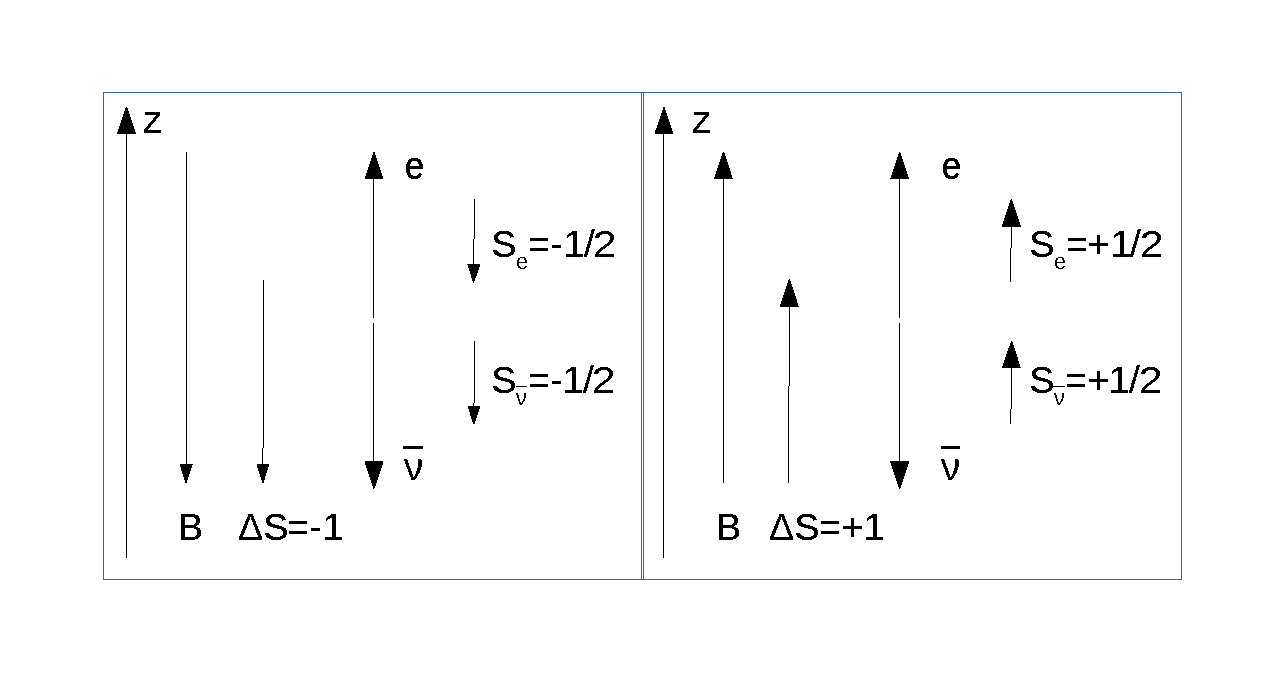
\includegraphics[width=0.6\linewidth]{DibujoExamen.pdf}
\end{center}
\caption{Visión esquemática del experimento de Madame Wu para dos configuraciones opuestas de campo magnético.}
\label{dibujo}
\end{figure}

\begin{figure}[!h]
\begin{center}
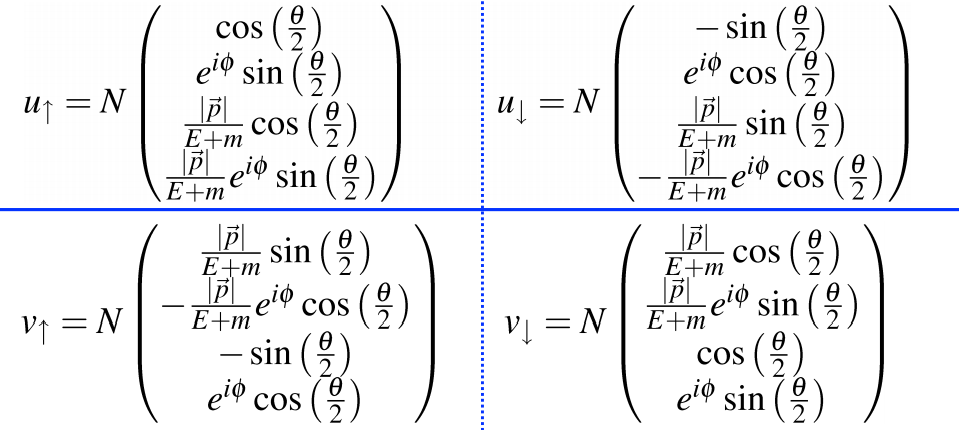
\includegraphics[width=0.6\linewidth]{espinores.png}
\end{center}
\caption{Espinores solución a la ecuación de Dirac y autoestados del operador helicidad.}
\label{espinores}
\end{figure}






\end{document}
